\title{Лекция 7\\Представление в базе знаний параметров и величин}   
\author[]{Шункевич Д.В.}
\institute[]{Белорусский государственный университет информатики и радиоэлектроники}

\begin{frame}
	\titlepage
\end{frame}

\begin{frame}{\\Содержание лекции}
	\topline
	\justifying
	Понятие шкалы, величины и параметра. Измеряемые и неизмеряемые параметры. Точные, неточные и интервальные величины. Связь с понятием мощности множества, бесконечного и конечного множества.
\end{frame}

%TODO Пример, подводящий к тому, что параметры нужны

\begin{frame}{\\Определение параметра}
	\topline
	\justifying
	\textbf{\textit{параметр}} -- класс, являющийся семейством всевозможных классов эквивалентности или толерантности, задаваемых либо отношением эквивалентности, либо отношением толерантности.\\		
\end{frame}

\begin{frame}{\\Определение параметра}
	\topline
	\justifying
	\begin{SCn}
		\scnheader{параметр}
		\scnidtf{характеристика}
		\scnidtf{свойство}
		\scnidtf{признак}		
		\scnidtf{измеряемое свойство}
		\scnidtf{класс классов}		
		\scnidtf{признак классификации или покрытия некоторого класса сущностей}
		\scnidtf{признак разбиения или покрытия некоторого класса сущностей}
		\scnidtf{семейство множеств, разбивающих или покрывающих некоторый класс сущностей}
		\scnidtf{семейство классов сущностей, обладающих одинаковым соответствующим свойством}
		\scnsuperset{ориентированный параметр}			
	\end{SCn}
\end{frame}

\begin{frame}{\\Типы параметров. Измеряемый параметр}
	\topline
	\justifying
	\begin{SCn}
		\scnheader{параметр}
		\begin{scnrelfromset}{\textit{разбиение}}
			\scnitem{измеряемый параметр}
			\scnitem{неизмеряемый параметр}
		\end{scnrelfromset}
	
		\scnheader{измеряемый параметр}
		\scnidtf{количественный параметр}
		\scnidtf{семейство измеряемых величин}
		\scntext{пояснение}{\footnotesize{Каждый \textbf{\textit{измеряемый параметр}} представляет собой \textit{параметр}, значение (элемент, экземпляр) которого трактуется как \textit{величина}, которой можно поставить в соответствие ее числовое значение на основании выбранной единицы измерения и/или точки отсчета (нулевой отметки выбранной шкалы).}}
		\scnsuperset{параметр, измеряемый по шкале}
		
	\end{SCn}
\end{frame}

\begin{frame}{\\Неизмеряемый параметр}
	\topline
	\justifying
	\begin{SCn}
		\scnheader{неизмеряемый параметр}
		\scnidtf{качественный параметр}
	\end{SCn}
	\textbf{\textit{неизмеряемый параметр}} -- это параметр, для которого нельзя подобрать числовой эквивалент и единицу измерения. Примеры: цвет, вкус.
\end{frame}

\begin{frame}{\\}
	\topline
	\justifying
	\begin{SCn}
		\scnheader{параметр}			
		\scntext{пояснение}{\small{Каждый \textbf{\textit{параметр}} представляет собой класс, являющийся семейством всевозможных классов эквивалентности или толерантности, задаваемых либо \textit{отношением эквивалентности}, либо \textit{отношением толерантности} (симметричным, рефлексивным, но частично транзитивным).
				
		Так, например, элементами (значениями, величинами) \textbf{\textit{параметра}} \textit{длина} являются либо классы эквивалентности, задаваемые отношением эквивалентности ``\textit{иметь точно одинаковую длину*}'', либо классы толерантности, задаваемые отношением вида ``\textit{иметь приблизительно одинаковую длину с указываемой точностью*}'', либо интервальные классы, задаваемые бинарными отношениями вида ``\textit{иметь длину, находящуюся в одном и том же указываемом интервале*}'' (например, от 1 метра до 2 метров).}}	 
	\end{SCn}
\end{frame}


\begin{frame}{\\Параметрическое пространство}
	\topline
	\justifying
	\begin{SCn}
		\scnheader{параметр}
		\scntext{пояснение}{\footnotesize{Заметим, что среди элементов (значений, величин) параметра могут встречаться пересекающиеся множества (классы), но объединение всех элементов каждого параметра есть не что иное, как класс всевозможных сущностей, обладающих этим параметром (свойством, характеристикой).
				
		Каждый конкретный параметр (характеристика), т.е. каждый элемент класса всевозможных параметров (характеристик) есть, по сути, признак классификации сущностей, обладающих это характеристикой, по принципу эквивалентности (одинаковости значения) этой характеристики. 
		
		Параметр может разбиваться на классы для уточнения некоторого свойства, например элементами параметра цвет будут классы, соответствующие конкретным цветам (синий, красный и т.д.), в свою очередь каждый конкретный цвет может включать более частные классы, уточняющие данное свойство, например, темно-синий, светло-красный и т.д.}
		}
	\end{SCn}
\end{frame}

\begin{frame}{\\Параметрическое пространство}
	\topline
	\justifying
	\begin{SCn}
		\scnheader{параметр}
		\scntext{пояснение}{\footnotesize{Другими словами, каждому множеству сущностей может ставиться в соответствие набор (семейство) параметров (параметрическое пространство), которыми обладают сущности этого множества -- аналог семейства отношений, определенных (заданных) на этом множестве. Часто бывает важно построить такое параметрическое пространство, "точки"{} которого взаимнооднозначно соответствуют параметризуемым сущностям (например, набор параметров, позволяющих однозначно идентифицировать, установить личность каждого человека).
						
		Таким образом, для каждого используемого элемента (значения) какого-либо параметра, необходимо явно указывать спецификацию этого значения (точное значение, неточное значение, интервальное значение, точность, интервал).}
		}
	\end{SCn}	
\end{frame}

\begin{frame}{\\Параметр. Примеры}
	\topline
	\justifying
	\vspace{10mm}
	\begin{figure}[H]
		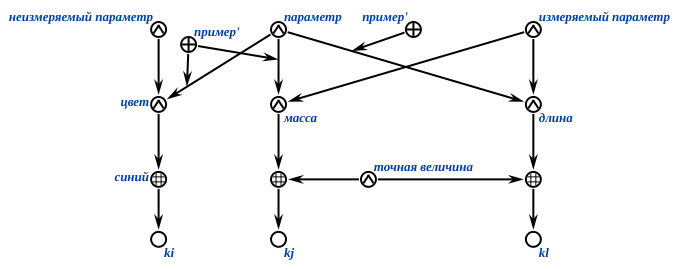
\includegraphics[scale=0.7]{./figures/sd_parameters/parameterDescription.png}
	\end{figure}
\end{frame}

\begin{frame}{\\Величина}
	\topline
	\justifying
	\begin{SCn}
		\scnheader{величина}
		\scnidtf{значение количественного параметра}
		\scnidtf{значение измеряемого параметра}
		\scnidtf{класс сущностей, имеющих одинаковое значение соответствующего параметра}
		\scnsuperset{точная величина}
		\scnsuperset{неточная величина}
		\scnsuperset{интервальная величина}
	\end{SCn}
\end{frame}

\begin{frame}{\\Величина}
	\topline
	\justifying
	\begin{SCn}
		\scnheader{величина}
		\scntext{пояснение}{\footnotesize{Каждая \textbf{\textit{величина}} представляет собой однозначный и независящий от шкалы измерения результат измерения некоторой характеристики у некоторой сущности.
			
		Каждой \textbf{\textit{величине}} можно поставить в соответствие ее числовое значение на основании выбранной единицы измерения и точки отсчета (нулевой отметки выбранной шкалы, в случае, если измерение осуществляется по шкале).
		
		Нельзя путать значение параметра (\textbf{\textit{величину}}) и значение величины по некоторой шкале, которое может быть скалярным и векторным.}		}
	\end{SCn}
\end{frame}

\begin{frame}{\\Отношение \textit{измерение*}}
	\topline
	\justifying
	\begin{SCn}
		\scnheader{измерение*}
		\scnidtf{значение параметра*}
		\scnidtf{значение заданной величины заданного параметра*}
		\scnidtf{измерение как соответствие*}
		\scnidtf{результат измерения заданной величины в заданной единице измерения и по заданной шкале*}
		\scnidtf{бинарное ориентированное отношение, связывающее различные величины с результатами их измерения в различных единицах измерения и по различным шкалам*}		
	\end{SCn}
\end{frame}

\begin{frame}{\\Отношение \textit{измерение*}}
	\topline
	\justifying
	\begin{SCn}
		\scnheader{измерение*}		
		\scntext{пояснение}{Связки отношения \textit{измерение*} связывают величину и ее значение в некоторой единице измерения (в том числе, в интервале) или по некоторой шкале.
			
		Конкретная единица измерения или шкала указывается дополнительно при помощи соответствующего отношения. Одной величине может соответствовать только одно значение в каждой возможной единице измерения или одна точка на некоторой шкале.}
	\end{SCn}
\end{frame}

\begin{frame}{\\Отношение \textit{точность*}}
	\topline
	\justifying
	\begin{SCn}
		\scnheader{точность*}
		\scnidtf{отклонение*}
		\scnidtf{степень точности неточного значения параметра*}
		\scniselement{бинарное отношение}
		\scntext{пояснение}{Связки отношения \textbf{\textit{точность*}} связывают \textit{неточную величину} и \textit{точную величину} того же класса, задающую максимальное возможное отклонение указанной \textit{неточной величины} от своего значения.}
	\end{SCn}
\end{frame}

\begin{frame}{\\Отношение \textit{единица измерения*}}
	\topline
	\justifying
	\begin{SCn}
		\scnheader{единица измерения*}
		\scniselement{бинарное отношение}
		\scnidtf{единица по шкале*}
		\scnidtf{единичная отметка по шкале*}
		\scntext{пояснение}{Связки отношения \textbf{\textit{единица измерения*}} связывают знак конкретного \textbf{\textit{измерения с фиксированной единицей измерения}} и некоторую \textit{точную величину}, входящую в тот же конкретный \textit{параметр}, что и первый компонент связок этого конкретного измерения, и которая используется в данном случае в качестве единицы измерения.}
	\end{SCn}
\end{frame}

\begin{frame}{\\ \small{Измерение с фиксированной единицей измерения}}
	\topline
	\justifying
	\begin{SCn}
		\scnheader{измерение с фиксированной единицей измерения }
		\scnrelto{семейство подмножеств}{измерение*}
		\scntext{пояснение}{Каждая \textbf{\textit{измерение с фиксированной единицей измерения}} представляет собой подмножество отношения \textit{измерение*} и характеризуется некоторой \textit{единицей измерения*}, которая является элементом того же параметра (семейством сущностей, имеющих значение данного параметра, совпадающее с этой единицей измерения).}
	\end{SCn}
\end{frame}

\begin{frame}{\\Измерение по шкале}
	\topline
	\justifying
	\begin{SCn}
		\scnheader{измерение по шкале}
		\scnidtf{шкала}
		\scnrelto{семейство подмножеств}{измерение*}
		\scntext{пояснение}{\small{Каждое \textbf{\textit{измерение по шкале}} представляет собой подмножество отношения \textit{измерение*} и характеризуется не единицей измерения, а некоторой точкой отсчета для данной \textbf{\textit{шкалы}}.
		
		Результатом \textbf{\textit{измерения по шкале}} будет некоторая точка шкалы, отстоящая от точки отсчета на определенное расстояние в нужную сторону (меньшую или большую). Понятно, что это расстояние может быть измерено любыми единицами измерения, но его величина при этом останется неизменной.}}
	\end{SCn}
\end{frame}

\begin{frame}{\\Измерение по шкале}
	\topline
	\justifying
	\begin{SCn}
		\scnheader{измерение по шкале}		
		\scntext{пояснение}{Не стоит путать измерение по \textbf{\textit{измерение по шкале}}, которое зависит от \textit{нулевой отметки*}, с измерением изменения того же \textit{параметра}, которое характеризуется единицей измерения и не зависит от точки отсчета. Например, не стоит путать дату по некоторому календарю, соответствующую \textit{началу} какого-либо процесса, и \textit{длительность} этого процесса, которая не зависит от выбранного календаря.}
	\end{SCn}
\end{frame}

\begin{frame}{\\Измерение по шкале. Нулевая отметка}
	\topline
	\justifying
	\begin{SCn}
		\scnheader{нулевая отметка*}
		\scnidtf{нуль по шкале*}
		\scnidtf{начало отсчета*}
		\scnidtf{точка отсчета*}
		\scniselement{бинарное отношение}		
		\scntext{пояснение}{Связки отношения \textbf{\textit{нулевая отметка*}} связывают знак некоторого \textit{измерения по шкале} со знаком \textit{точной величины} того же \textit{параметра}, которая в рамках данной шкалы принимается за точку отсчета.}
	\end{SCn}
\end{frame}

\begin{frame}{\\Измерение по шкале. Пример}
	\topline
	\justifying
	\vspace{10mm}
	\begin{figure}[H]
		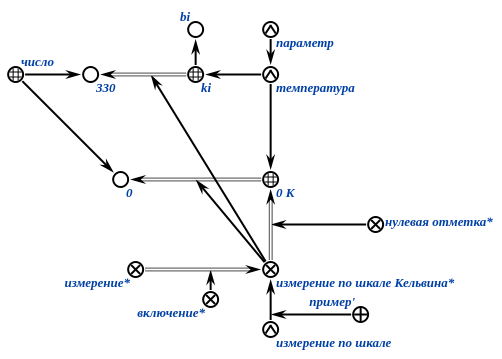
\includegraphics[scale=0.7]{./figures/sd_parameters/scale.png}
	\end{figure}
\end{frame}

\begin{frame}{\\Точная величина}
	\topline
	\justifying
	\begin{SCn}
		\scnheader{точная величина}
		\scnidtf{точное значение параметра}
		\scnidtf{множество всех точных значений параметра}
		\scnidtf{значение параметра, являющееся семейством классов эквивалентности, соответствующим некоторому отношению эквивалентности}
		\scnidtf{класс эквивалентности}
		\scntext{пояснение}{\footnotesize{Каждая \textbf{\textit{точная величина}} имеет одно фиксированное значение в некоторой единице измерения или по какой-либо шкале. При этом считается, что все элементы такого класса имеют одинаковое значение данного параметра и отклонениями можно пренебречь.
				
		Каждой \textbf{\textit{точной величине}} можно поставить в соответствие группу \textit{неточных величин}, являющихся не разбиениями, а покрытиями того же множества, но с разной степенью точности.}}
	\end{SCn}
\end{frame}

\begin{frame}{\\Точная величина. Пример}
	\topline
	\justifying
	\vspace{10mm}
	\begin{figure}[H]
		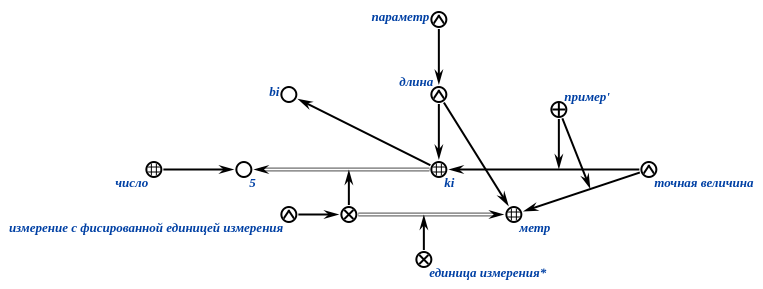
\includegraphics[scale=0.6]{./figures/sd_parameters/exactLength.png}
	\end{figure}
\end{frame}

\begin{frame}{\\Неточная величина}
	\topline
	\justifying
	\begin{SCn}
		\scnheader{неточная величина}
		\scnidtf{множество неточных значений параметра}
		\scnidtf{приблизительная величина}
		\scnidtf{приблизительное значение параметра}
		\scnidtf{значение параметра в интервале с нефиксированными границами}
		\scntext{пояснение}{\small{Каждой \textbf{\textit{неточной величине}} ставится в соответствие ее значение в некоторой единице измерения или по какой-либо шкале, а также дополнительно указывается \textit{точность*}, т.е. возможное отклонение от данного значения.}}
	\end{SCn}
\end{frame}

\begin{frame}{\\Неточная величина. Пример}
	\topline
	\justifying
	\vspace{10mm}
	\begin{figure}[H]
		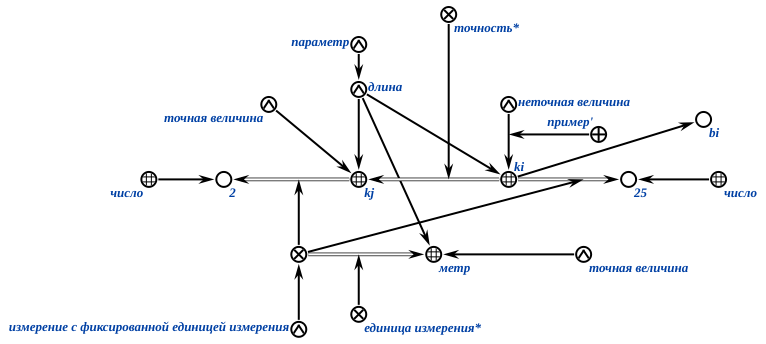
\includegraphics[scale=0.6]{./figures/sd_parameters/approximateLength.png}
	\end{figure}
\end{frame}

\begin{frame}{\\Интервальная величина}
	\topline
	\justifying
	\begin{SCn}
		\scnheader{интервальная  величина}
		\scnidtf{интервальное значение параметра}
		\scnidtf{значение параметра в интервале с фиксированными границами}
		\scnidtf{интервал значения параметра из множества пересекающихся интервалов разной длины, имеющих нефиксированные границы}
		\scntext{пояснение}{\small{Каждая \textbf{\textit{интервальная величина}} представляет собой класс сущностей, находящихся в рамках точно заданного интервала, минимальная и максимальная точка которого являются \textit{точными величинами}. Результатом \textit{измерения*} такой величины является ориентированная пара, первым компонентом которой является левая (меньшая) граница интервала, вторым компонентом -- правая (большая) граница интервала.}}
	\end{SCn}
\end{frame}

\begin{frame}{\\Интервальная величина. Пример}
	\topline
	\justifying
	\vspace{10mm}
	\begin{figure}[H]
		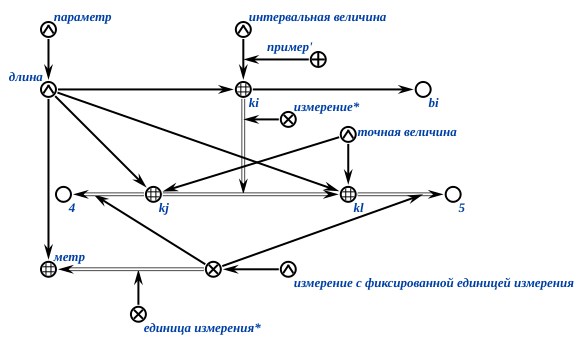
\includegraphics[scale=0.7]{./figures/sd_parameters/intervalLength.png}
	\end{figure}
\end{frame}

\begin{frame}{\\Измерение как действие}
	\topline
	\justifying
	\begin{SCn}
		\scnheader{действие. измерение}
		\scnidtf{измерение как действие}
		\scnidtf{действие, направленное на установление связи, принадлежащей отношению измерение* и связывающей величину, которая принадлежит заданному параметру, и которой принадлежит заданная сущность, и соответствующее значение этой величины на некоторой шкале}
		\scnidtf{действие, направленное на решение задачи измерения заданного параметра у заданной сущности}
		\scnsubset{действие}		
	\end{SCn}
\end{frame}

\begin{frame}{\\Измерение как задача}
	\topline
	\justifying
	\begin{SCn}				
		\scnheader{задача. измерение}
		\scnidtf{спецификация действия измерения}
		\scnidtf{спецификация действия, целью которого является измерение заданного параметра у заданной сущности}
		\scnsubset{задача}
	\end{SCn}
\end{frame}

